\apendice{Especificación de Requisitos}

\section{Introducción}
En esta sección se abordarán los diferentes objetivos y requisitos del proyecto. Se presentarán tanto los requisitos globales del proyecto, como los requisitos funcionales y casos de uso de la aplicación.

\section{Objetivos generales}
\begin{itemize}
    \item Realizar una exhaustiva investigación sobre los algoritmos de comparación de secuencias temporales, para comprobar el inicio y el final de éstas en otras secuencias.
    \item Investigar múltiples librerías en \textit{Python} que permitan la localización de secuencias multidimensionales lo más parecidas posible a un patrón de referencia, dentro de una secuencia de mayor tamaño.
    \item Investigar y analizar como se podría clasificar un ejercicio según las partes del cuerpo que estén en movimiento.
    \item Recopilación de vídeos adecuados para la investigación, tanto para ser empleados en este proyecto como en proyectos futuros, comprobando que son idóneos para su análisis. 
    \item Realizar una aplicación de escritorio por la cual se pueda observar un recorte de un ejercicio concreto de un vídeo con múltiples ejercicios.
\end{itemize}

\section{Catalogo de requisitos}

\subsection{Requisitos del proyecto}

Para ejecutar el programa correctamente se necesitan una serie de requisitos \textit{software} y \textit{hardware}.


\textbf{Requisitos \textit{software}}
\begin{enumerate}
    \item Consola Unix o macOS.
    \item \textit{Python 3}.
    \item Instalación drivers de \textit{CUDA}, versión de 9.2 a 11.2.
    \item Librerías:
    \begin{enumerate}
        \item \textit{Numpy}, 1.20.0.
        \item \textit{Pickle}, 0.7.5.
        \item \textit{Pandas}, 1.0.1.
        \item \textit{OpenCV} (cv2), 4.5.5.62.
        \item \textit{Garbage Collector} (gc).
        \item Librería de manejo \textit{NVIDIA} (pynvml), 11.4.1.
        \item \textit{Matplotlib}, 3.2.0.
        \item \textit{Seaborn}, 0.11.2.
        \item \textit{Plotly}.
        \item \textit{PyTorch} (torch), 1.9.0+cu111.
        \item \textit{Torchvision}, 0.10.0+cu111.
        \item \textit{Math}, 1.2.1.
        \item \textit{Os}, 3.10.5.
        \item \textit{tensorflow}, 2.8.0.
        \item \textit{Detectron2}, 0.6.
        \item \textit{pydtw}, 2.0.2.
        \item \textit{tslearn}, 0.5.2.
        \item \textit{scipy}, 1.4.1.
        \item \textit{Dtaidistance}, 2.3.6.
    \end{enumerate}

\end{enumerate}

\textbf{Requisitos \textit{hardware}}
\begin{enumerate}
    \item Tarjeta gráfica con drivers CUDA con al menos 1GB de memoria.
\end{enumerate}

\subsection{Requisitos de la aplicación}

En este apartado se mostrarán los requisitos funcionales de la aplicación de escritorio. Aunque ha sido creada para comprobar los resultados de las ejecuciones, esta aplicación también podría ser usada por un terapeuta que quiere observar como de bien están realizando sus pacientes los ejercicios prescritos.  

\textbf{Actores}
\begin{enumerate}
    \item \emph{Terapeuta}: este actor será el que utilice la aplicación. Idealmente será el terapeuta correspondiente al paciente del que se están analizando los vídeos.
    \item \emph{Científico de datos}: este actor será quien manipule los ficheros que procesan las secuencias y le pasará al terapeuta los \textit{frames} de inicio y final de la secuencia. Este actor no intervendrá con la aplicación por lo que no recibirá un diagrama de uso. 
    \item \emph{Usuario}: este actor será un miembro del tribunal o cualquier otro individuo que quiera comprobar de una forma visual la finalidad del proyecto sin tener que ejecutarle.
\end{enumerate}

En este apartado se mostrarán los requisitos funcionales del proyecto la aplicación.
\begin{itemize}
	\item \textbf{RF.1} Manipulación de vídeos. 
	\begin{itemize}
	\item \textbf{RF.1.1} El terapeuta podrá seleccionar el vídeo que quiere localizar.
	\item \textbf{RF.1.2} El terapeuta podrá seleccionar el vídeo en el que quiere que se localice el ejercicio concreto. 
	\item \textbf{RF.1.3} El usuario podrá seleccionar el vídeo que quiere localizar.
	\item \textbf{RF.1.4} El usuario podrá seleccionar el vídeo en el que quiere que se localice el ejercicio concreto.
	\end{itemize}
	
	\item \textbf{RF.2} Visualización de vídeos tanto del terapeuta como del paciente.
	\begin{itemize}
	\item \textbf{RF.2.1} El terapeuta podrá reproducir el vídeo concreto.
	\item \textbf{RF.2.2} El terapeuta podrá reproducir el vídeo que contiene todos los ejercicios.
	\item \textbf{RF.2.3} El terapeuta podrá pausar el vídeo concreto.
	\item \textbf{RF.2.4} El terapeuta podrá pausar el vídeo que contiene todos los ejercicios.
	\item \textbf{RF.2.5} El usuario podrá reproducir el vídeo concreto.
	\item \textbf{RF.2.6} El usuario podrá reproducir el vídeo que contiene todos los ejercicios.
	\item \textbf{RF.2.7} El usuario podrá pausar el vídeo concreto.
	\item \textbf{RF.2.8} El usuario podrá pausar el vídeo que contiene todos los ejercicios.
	\end{itemize}
	
	\item \textbf{RF.3} Visualización de resultados.
	\begin{itemize}
	\item \textbf{RF.3.1} El terapeuta podrá reproducir el vídeo resultante.
	\item \textbf{RF.3.2} El terapeuta podrá pausar el vídeo resultante.
	\item \textbf{RF.3.3} El terapeuta podrá indicar el \textit{frame} en el que se inicia el vídeo.
	\item \textbf{RF.3.4} El terapeuta podrá indicar el \textit{frame} en el que se finaliza el vídeo.
	\item \textbf{RF.3.5} El usuario podrá reproducir el vídeo resultante.
	\item \textbf{RF.3.6} El usuario podrá pausar el vídeo resultante.
	\end{itemize}
	
	\item \textbf{RF.4} Gestión de vídeos: carga, eliminación
	\begin{itemize}
    \item \textbf{RF.4.1} El terapeuta podrá introducir en el directorio que contiene los vídeos concretos todos los vídeos que desee analizar.
	\item \textbf{RF.4.2} El terapeuta podrá introducir en el directorio que contiene los vídeos completos todos los vídeos que desee analizar.
	\item \textbf{RF.4.3} El usuario podrá introducir en el directorio que contiene los vídeos concretos todos los vídeos que desee analizar.
	\item \textbf{RF.4.4} El usuario podrá introducir en el directorio que contiene los vídeos completos todos los vídeos que desee analizar.
	\end{itemize}
	
	\item \textbf{RF.5} Gestión de resultados: almacenamiento.
	\begin{itemize}
	\item \textbf{RF.5.1} El terapeuta podrá guardar el vídeo resultante. 
	\end{itemize}
	
	\item \textbf{RF.6} Comprobación de resultados en distintos modos de ejecución.
	\begin{itemize}
	\item \textbf{RF.6.1} El terapeuta podrá cambiar al entre el modo de ejemplo y el modo de ejecución. 
	\item \textbf{RF.6.2} El usuario podrá cambiar al entre el modo de ejemplo y el modo de ejecución.
	\item \textbf{RF.6.3} El usuario podrá observar un recorte del ejercicio sin seleccionar el \textit{frame} de inicio.
	\item \textbf{RF.6.4} El usuario podrá observar un recorte del ejercicio sin seleccionar el \textit{frame} de final.
	\end{itemize}
\end{itemize}


\section{Especificación de requisitos}

En este apartado se van a mostrar, por una parte los diagramas de casos de uso, como se puede observar en las figuras  \ref{f:casoUsoTerapeuta} y \ref{f:casoUsoUsuario} y por otra, las tablas de casos de uso. 

La única diferencia que muestra la aplicación entre el \textit{modo ejemplo ON} y el \textit{modo ejemplo OFF}, es que en este último caso se deberán de especificar los \textit{frames} de inicio y de final.


\begin{figure}[H]
 \centering
\subfloat{
    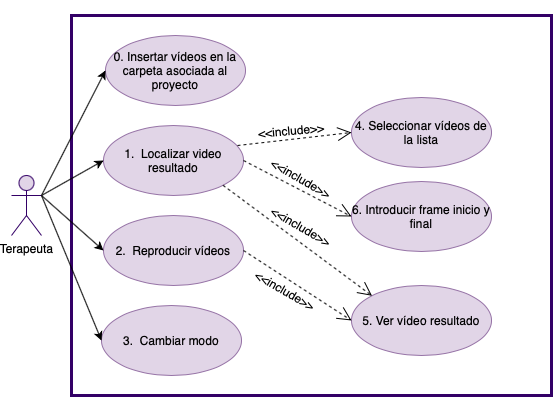
\includegraphics[width=\textwidth]{plantillaLatex-master/img/DiagramaUsoTera copia.png}}
 \caption{Diagrama de casos de uso para el terapeuta.}
 \label{f:casoUsoTerapeuta}
\end{figure}

\begin{figure}[H]
 \centering
  \subfloat{
    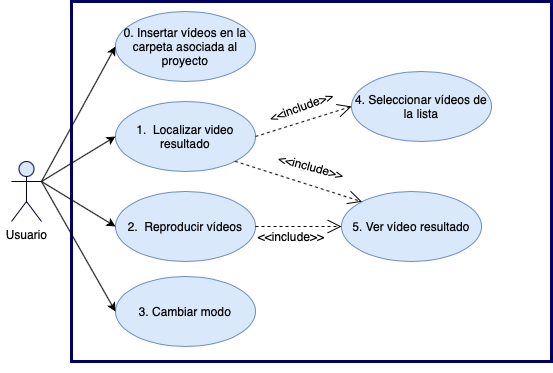
\includegraphics[width=\textwidth]{DiagramaUsoUser.png}}
 \caption{Diagrama de casos de uso para el usuario.}
 \label{f:casoUsoUsuario}
\end{figure}


\tablaSmallSinColores{Caso de uso 0: Insertar vídeos.}{p{3cm} p{.75cm} p{8.5cm}}{tablaUC0}{
  \multicolumn{3}{l}{Caso de uso 0: Insertar vídeos.} \\
 }
 {
  Descripción                            & \multicolumn{2}{p{10.25cm}}{Permite al usuario cargar vídeos de su equipo a la aplicación.} \\\hline
  \multirow{2}{3.5cm}{Requisitos}   &\multicolumn{2}{p{10.25cm}}{RF-4.1} \\\cline{2-3}
                                         & \multicolumn{2}{p{10.25cm}}{RF-4.2} \\\cline{2-3}
                                         & \multicolumn{2}{p{10.25cm}}{RF-4.3} \\\cline{2-3}
                                         & \multicolumn{2}{p{10.25cm}}{RF-4.4}
                                         \\\hline
  Precondiciones                         &  \multicolumn{2}{p{10.25cm}}{Ninguna}   \\\hline
  \multirow{2}{3.5cm}{Secuencia normal}  & Paso & Acción \\\cline{2-3}
                                         & 1    & El usuario o terapeuta introducen los vídeos en el directorio deseado.
  \\\cline{2-3}
                                         & 2    & Al ejecutar la aplicación los vídeos se cargan automáticamente en la barra de selección.
                                         \\\hline
  Postcondiciones                        & \multicolumn{2}{p{10.25cm}}{Vídeos aparecen en cada una de sus listas de selección para posteriormente poder ser mostrados.} \\\hline
  Excepciones                        & \multicolumn{2}{p{10.25cm}}{Ninguna}\\\hline
  Importancia                            & Alta \\\hline
  Urgencia                               & Alta \\
}

\tablaSmallSinColores{Caso de uso 1: Localiza el vídeo.}{p{3cm} p{.75cm} p{8cm}}{tablaUC1}{
  \multicolumn{3}{l}{Caso de uso 1: Localiza el vídeo.} \\
 }
 {
  Descripción                            & \multicolumn{2}{p{10.25cm}}{Permite al usuario localizar el vídeo concreto dentro del vídeo que contiene múltiples ejercicios.} \\\hline
  \multirow{2}{3.5cm}{Requisitos}   &\multicolumn{2}{p{10.25cm}}{RF-1.1} \\\cline{2-3}
                                         & \multicolumn{2}{p{10.25cm}}{RF-1.2} \\\cline{2-3}
                                         & \multicolumn{2}{p{10.25cm}}{RF-1.3} \\\cline{2-3}
                                         & \multicolumn{2}{p{10.25cm}}{RF-1.4} \\\cline{2-3}
                                         \\\hline
  Precondiciones                         &  \multicolumn{2}{p{10.25cm}}{Tener por lo menos algún vídeo concreto y algún vídeo completo cargado}   \\\hline
  \multirow{2}{3.5cm}{Secuencia normal}  & Paso & Acción \\\cline{2-3}
                                         & 1    & El usuario o terapeuta seleccionan el vídeo concreto deseado. \\\cline{2-3}
                                         & 2    & El usuario o terapeuta seleccionan el botón mostrar. \\\cline{2-3}
                                         & 3    & El usuario o terapeuta seleccionan el vídeo concreto deseado. \\\cline{2-3}
                                         & 4    & El usuario o terapeuta seleccionan el botón mostrar. \\\cline{2-3}
                                         & 5    & El usuario o terapeuta seleccionan el botón recortar.\\\cline{2-3}
                                         & 4    & Aparece el vídeo recortado. 
                                         \\\hline
  Postcondiciones                        & \multicolumn{2}{p{10.25cm}}{El vídeo localizado se reproduce automáticamente en la aplicación y se guarda una copia del mismo en la carpeta en la que se ejecuta el proyecto.} \\\hline
  Excepciones                        & \multicolumn{2}{p{10.25cm}}{Ninguna}\\\hline
  Importancia                            & Alta \\\hline
  Urgencia                               & Alta \\
}

\tablaSmallSinColores{Caso de uso 2: Reproducir vídeos.}{p{3cm} p{.75cm} p{8.5cm}}{tablaUC2}{
  \multicolumn{3}{l}{Caso de uso 2: Reproducir vídeos.} \\
 }
 {
  Descripción                            & \multicolumn{2}{p{10.25cm}}{Permite al usuario reproducir y pausar los diferentes vídeos.} \\\hline
  \multirow{2}{3.5cm}{Requisitos}   &\multicolumn{2}{p{10.25cm}}{RF-2.1} \\\cline{2-3}
                                         & \multicolumn{2}{p{10.25cm}}{RF-2.2} \\\cline{2-3}
                                         & \multicolumn{2}{p{10.25cm}}{RF-2.3} \\\cline{2-3}
                                         & \multicolumn{2}{p{10.25cm}}{RF-2.4} \\\cline{2-3}
                                         & \multicolumn{2}{p{10.25cm}}{RF-2.5} \\\cline{2-3}
                                         & \multicolumn{2}{p{10.25cm}}{RF-2.6} \\\cline{2-3}
                                         & \multicolumn{2}{p{10.25cm}}{RF-2.7} \\\cline{2-3}
                                         & \multicolumn{2}{p{10.25cm}}{RF-2.8}
                                         \\\hline
  Precondiciones                         &  \multicolumn{2}{p{10.25cm}}{Tener el vídeo que se desea reproducir o pausar cargado.}   \\\hline
  \multirow{2}{3.5cm}{Secuencia normal}  & Paso & Acción \\\cline{2-3}
                                         & 1    & El usuario o terapeuta seleccionan un vídeo.
  \\\cline{2-3}
                                         & 2    & El usuario o terapeuta pincha sobre el botón play.\\\cline{2-3}
                                         & 3    & Vídeo comienza a reproducirse.\\\cline{2-3}
                                         & 4    & El usuario o terapeuta puede pinchar sobre el botón pause.\\\cline{2-3}
                                         & 5    & El usuario o terapeuta puede pinchar sobre el botón stop.\\\cline{2-3}
                                         & 6    & El vídeo se para.
                                         \\\hline
  Postcondiciones                        & \multicolumn{2}{p{10.25cm}}{Ninguna.} \\\hline
  Excepciones                        & \multicolumn{2}{p{10.25cm}}{Ninguna}\\\hline
  Importancia                            & Alta \\\hline
  Urgencia                               & Alta \\
}

\tablaSmallSinColores{Caso de uso 3: Cambiar modo.}{p{3cm} p{.75cm} p{8.5cm}}{tablaUC3}{
  \multicolumn{3}{l}{Caso de uso 3: Cambiar modo.} \\
 }
 {
  Descripción                            & \multicolumn{2}{p{10.25cm}}{Permite al usuario o al terapeuta cambiar el modo de la aplicación.} \\\hline
  \multirow{2}{3.5cm}{Requisitos}   &\multicolumn{2}{p{10.25cm}}{RF-6.1} \\\cline{2-3}
                                         & \multicolumn{2}{p{10.25cm}}{RF-6.2} \\\cline{2-3}
                                         & \multicolumn{2}{p{10.25cm}}{RF-6.3} \\\cline{2-3}
                                         & \multicolumn{2}{p{10.25cm}}{RF-6.4}
                                         \\\hline
  Precondiciones                         &  \multicolumn{2}{p{10.25cm}}{Ninguna}   \\\hline
  \multirow{2}{3.5cm}{Secuencia normal}  & Paso & Acción \\\cline{2-3}
                                         & 1    & El usuario o terapeuta seleccionan el botón de cambio de modo.
  \\\cline{2-3}
                                         & 2    & Se cambia el modo de la pantalla. 
                                         \\\hline
  Postcondiciones                        & \multicolumn{2}{p{10.25cm}}{Se habilitan o deshabilitan las casillas de los \textit{frames}, se actualizan los vídeos y se cambian los colores.} \\\hline
  Excepciones                        & \multicolumn{2}{p{10.25cm}}{Ninguna}\\\hline
  Importancia                            & Alta \\\hline
  Urgencia                               & Alta \\
}

\tablaSmallSinColores{Caso de uso 4: Seleccionar vídeos de la lista.}{p{3cm} p{.75cm} p{8.5cm}}{tablaUC4}{
  \multicolumn{3}{l}{Caso de uso 4: Seleccionar vídeos de la lista.} \\
 }
 {
  Descripción                            & \multicolumn{2}{p{10.25cm}}{Permite al usuario o terapeuta seleccionar los vídeos concretos o completos que desea reproducir.} \\\hline
  \multirow{2}{3.5cm}{Requisitos}   &\multicolumn{2}{p{10.25cm}}{RF-1.2} \\\cline{2-3}
                                         & \multicolumn{2}{p{10.25cm}}{RF-1.2} \\\cline{2-3}
                                         & \multicolumn{2}{p{10.25cm}}{RF-1.3} \\\cline{2-3}
                                         & \multicolumn{2}{p{10.25cm}}{RF-1.4}
                                         \\\hline
  Precondiciones                         &  \multicolumn{2}{p{10.25cm}}{Que la lista contenga vídeos.}   \\\hline
  \multirow{2}{3.5cm}{Secuencia normal}  & Paso & Acción \\\cline{2-3}
                                         & 1    & El usuario o terapeuta seleccionarán un vídeo concreto de la lista.\\\cline{2-3}
                                         & 2    & El usuario o terapeuta pincha sobre el botón añadir.\\\cline{2-3}
                                         & 3    & El vídeo se carga y se reproduce automáticamente.\\\cline{2-3}
                                         & 4    & El usuario o terapeuta seleccionarán un vídeo completo de la lista.\\\cline{2-3}
                                         & 5    & El usuario o terapeuta pincha sobre el botón añadir.\\\cline{2-3}
                                         & 6    & El vídeo se carga y se reproduce automáticamente.
                                         \\\hline
  Postcondiciones                        & \multicolumn{2}{p{10.25cm}}{Se muestran ambos vídeos cargados y reproduciéndose automáticamente hasta su finalización.} \\\hline
  Excepciones                        & \multicolumn{2}{p{10.25cm}}{Ninguna}\\\hline
  Importancia                            & Alta \\\hline
  Urgencia                               & Alta \\
}

\tablaSmallSinColores{Caso de uso 5: Ver vídeo resultado.}{p{3cm} p{.75cm} p{8.5cm}}{tablaUC5}{
  \multicolumn{3}{l}{Caso de uso 5: Ver vídeo resultado.} \\
 }
 {
  Descripción                            & \multicolumn{2}{p{10.25cm}}{Permite al usuario o terapeuta ver el vídeo final generado.} \\\hline
  \multirow{2}{3.5cm}{Requisitos}   &\multicolumn{2}{p{10.25cm}}{RF-6.3} \\\cline{2-3}
                                         & \multicolumn{2}{p{10.25cm}}{RF-6.4} \\\cline{2-3}
                                         & \multicolumn{2}{p{10.25cm}}{RF-5.1} \\\cline{2-3}
                                         & \multicolumn{2}{p{10.25cm}}{RF-3.1} \\\cline{2-3}
                                         & \multicolumn{2}{p{10.25cm}}{RF-3.2} \\\cline{2-3}
                                         & \multicolumn{2}{p{10.25cm}}{RF-3.5} \\\cline{2-3}
                                         & \multicolumn{2}{p{10.25cm}}{RF-3.6} 
                                         \\\hline
  Precondiciones                         &  \multicolumn{2}{p{10.25cm}}{Haber seleccionado tanto un vídeo concreto como completo. En el caso de no estar en el modo ejemplo será necesario indicar los \textit{frames} por los que se recorta.}   \\\hline
  \multirow{2}{3.5cm}{Secuencia normal}  & Paso & Acción \\\cline{2-3}
                                         & 1    & El usuario o terapeuta seleccionarán un vídeo concreto de la lista.\\\cline{2-3}
                                         & 2    & El usuario o terapeuta seleccionarán un vídeo completo de la lista.\\\cline{2-3}
                                         & 3    & En caso de que sea necesario se especifican los \textit{frames} de inicio y final.\\\cline{2-3}
                                         & 4    & Se pulsa el botón recortar.\\\cline{2-3}
                                         & 5    & El vídeo recortado se guarda automáticamente.
                                         \\\hline
  Postcondiciones                        & \multicolumn{2}{p{10.25cm}}{El vídeo recortado se muestra en la aplicación y se reproduce automáticamente.} \\\hline
  Excepciones                        & \multicolumn{2}{p{10.25cm}}{En caso de que sea necesario especificar el \textit{frame} de inicio y final y no se haya especificado informará del error.}\\\hline
  Importancia                            & Alta \\\hline
  Urgencia                               & Alta \\
}

\tablaSmallSinColores{Caso de uso 6: Introducir \textit{frames} de inicio y final.}{p{3cm} p{.75cm} p{8.5cm}}{tablaUC6}{
  \multicolumn{3}{l}{Caso de uso 6: Introducir \textit{frames} de inicio y final.} \\
 }
 {
  Descripción                            & \multicolumn{2}{p{10.25cm}}{Permite al terapeuta indicar el \textit{frame} de inicio y final del vídeo.} \\\hline
  \multirow{2}{3.5cm}{Requisitos}   &\multicolumn{2}{p{10.25cm}}{RF-3.3} \\\cline{2-3}
                                         & \multicolumn{2}{p{10.25cm}}{RF-3.4} 
                                         \\\hline
  Precondiciones                         &  \multicolumn{2}{p{10.25cm}}{Haber seleccionado tanto un vídeo concreto como completo. }   \\\hline
  \multirow{2}{3.5cm}{Secuencia normal}  & Paso & Acción \\\cline{2-3}
                                         & 1    & El terapeuta seleccionarán un vídeo concreto de la lista.\\\cline{2-3}
                                         & 2    & El terapeuta seleccionarán un vídeo completo de la lista.\\\cline{2-3}
                                         & 3    & El terapeuta especifica los \textit{frames} de inicio y final.\\\cline{2-3}
                                         & 4    & Se pulsa el botón recortar.\\\cline{2-3}
                                         & 5    & El vídeo recortado se guarda automáticamente.
                                         \\\hline
  Postcondiciones                        & \multicolumn{2}{p{10.25cm}}{El vídeo recortado se muestra en la aplicación y se reproduce automáticamente.} \\\hline
  Excepciones                        & \multicolumn{2}{p{10.25cm}}{Ninguna.}\\\hline
  Importancia                            & Alta \\\hline
  Urgencia                               & Alta \\
}

